\documentclass[a4paper]{article}

\usepackage[english]{babel}
\usepackage[utf8]{inputenc}
\usepackage{amsmath}
\usepackage{graphicx}
\usepackage[left=1in, right=1in, top=1in, bottom=1in]{geometry}
\usepackage{url}
\usepackage{wrapfig}

\title{Characterizing $\beta$ and Other Topics in SpMV Error Analysis}

\author{Melvyn Ian Drag}

\date{\today}

\begin{document}
\maketitle

\begin{abstract}
Iterated sparse matrix vector multiplication underlies many partial differential equation solvers. The size of the involved matrices is often quite large, and the products must be carried out supercomputers which produce non-halting, computation invalidating, ``soft errors". In this paper a brief description of three iterative solvers is provided, two methods of error analysis are introduced and compared, and an accepted means of error detection is expanded upon. Then, two important topics which cannot be covered in this paper are introduced to the reader in case he or she may be looking for further reading.
\end{abstract}


\section{Why Soft Error Detection Is Important to You}
You are a mathematician, a scientist, or a computer programmer who for some reason or other is involved with computational partial differential equations. You find yourself performing iterated matrix multiplication as a result of the transformation of continuous PDEs into matrix equations, and it is very important that your solution be as accurate as possible within the confines of floating point error.
\subsection{Soft Errors}
A soft error is an error in computation which will not cause the machine halt computation, but which can still silently destroy the validity of a computation. Soft errors are a serious issue in scientific computing because supercomputers make use of many small processors which run for extensive periods of time. While the frequency of error in a single processor is negligible, in a large system the laws of probability virtually guarantee that soft errors \emph{will} occur and \emph{will occur frequently}. These soft errors are typically bit flips or incorrect memory reads and writes which can generate single errors of arbitrarily high magnitude.
\begin{wrapfigure}{r}{0.5\textwidth}
  \begin{center}
    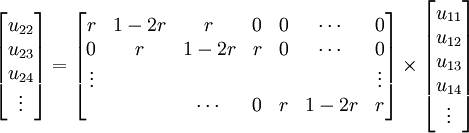
\includegraphics[width=0.48\textwidth]{heat_matrix.png}
  \end{center}
  \caption{The Discretization Matrix}
\end{wrapfigure}
\subsection{The Euler Method With Dirichlet Boundary Conditions}
This is the simplest of all of the iterative solvers. We will investigate this method via the heat equation.
\begin{equation}
u_t = u_{xx}
\end{equation}
This is the statement of the heat equation. To solve this equation in one dimension we will consider a heated metal bar. The temperature in the bar will try to reach some equilibrium depending on what sort of details we impose on the problem. Let us imagine that the bar is of length $\pi$, and let us furthermore imagine that the temperature in the ends of the bar is held fixed at zero degrees. This leads us to assume that $e^{-t}\sin(x)$ ought to be a good approximation of the temperature distribution in the bar, because it gives zero at $0$ and at $\pi$. Also, the exponential term will decay as time passes, and our experience in life is that heated things get cooler when they touch something held at a constant zero degrees. We check to see if our proposed solution is a solution to equation (1), and indeed it is.
\begin{gather}
u_t = u_{xx}\\
-e^{-t}sin(x) = e^{-t}(-sin(x))
\end{gather}

Then we realize that the bar is continuous, but that computers can't solve continuous problems, they can only give discrete approximations. 
so, we divide the bar up into small intervals, say by cutting the bar up with $n+1$ evenly spaced points. Say these points are spaced at a distance of $\Delta x$. Then we say that the equation we are trying to solve can be discretized as follows:
\begin{gather}
u_t = u_{xx}\\
\frac{u(x, t + \Delta t) - u(x, t)}{\Delta t} = \frac{u(x + \Delta x, t) - 2u(x, t) + u(x - \Delta x, t)}{\Delta x^2}\\
u(x, t + \Delta t) = u(x, t) + \frac{\Delta t}{\Delta x ^2}(u(x + \Delta x, t) - 2u(x, t) + u(x - \Delta x, t))
\end{gather}

And this lends itself to a matrix equation, because we have an equation for every point in the mesh, which combines a point at time step $t$ with its neighbors in a certain combination, and yields the value of the solution for the next step. We do not need to update the boundaries of the bar, because they are fixed at $0$. The matrix equation is in figure 1\footnote{Image from \url{https://source.ggy.bris.ac.uk/wiki/NumMethodsPDEs}}:

 It is easier to envision this equation with a mesh. The vertical axis represents the time step and the horizontal axis represents our metal bar. The temperature in the bar is in the z direction. Consider the following images.\footnote{Images from \url{http://en.wikipedia.org/wiki/Finite_difference_method} and \url{http://www.mathworks.com/help/matlab/math/pdepe1.gif}}
 
\begin{wrapfigure}{l}{0.4\textwidth}
\begin{center}
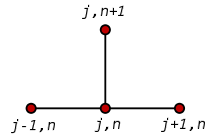
\includegraphics[width=0.4\textwidth]{forward.png}
\caption{The coordinates at time step n give a coordinate at time step n+1.}
\vspace{10pt}
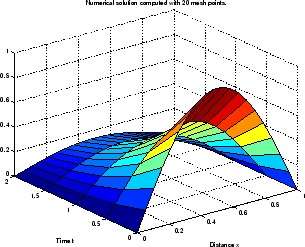
\includegraphics[scale = 0.4]{heat.jpg}
\caption{Here we see the bar in one direction, time passing in  the other direction, and the temperature (z axis) in the bar dropping as time passes.}
\end{center}
\vspace{-100pt}
\end{wrapfigure}

\emph{Skim the following information, do not worry about it. The importance of the row norm is coming up in a few pages.} Now notice that the maximum 2 norm of the rows of this equation is 
\begin{align}
||T_{row}||_{2, max}&=\sqrt{r^2 + (1-2r)^2 + r ^ 2}\\
&=\sqrt{r^2 + 1 - 4r + 4r^2 + r^2}\\
&=\sqrt{6r^2 - 4r + 1}
\end{align}
And we are interested in when this 2 norm is greater than one.
\begin{gather}
6r^2 - 4r + 1 = 1\\
6r^2 - 4r = 0\\
6r = 4\\
r = \frac23
\end{gather}
So the row norm is greater then one when $r$ is above $\frac23$
Also review equation (6) above and notice the $\Delta x $ and $\Delta t$ terms. These terms cannot be chosen randomly. There is a way to determine if your choice for these variables is numerically stable or not, and we will cover this shortly.
\subsection{The Euler Method With Neumann Boundary Conditions}
In the previous example we considered the ends of the bar being held at a constant temperature. We can specifiy the boundary values in a number of ways. Another popular way to choose the boundary conditions is to allow them to have a constant \emph{derivative}. Say we want the derivative on the boundary to equal zero at all times, we can let our solution $u(x, t) = e^{-t}cos(x)$. Computing the derivatives and plugging into equation (2) will show that this is indeed a solution to the equation. The interior points can be calculated in the same way, and we see that $u'(x,t) = 0$
on the boundary, as we want. (Remember that the domain is $[0, \pi]$).
We only need to change the top and bottom rows of the matrix using the subsitution :
\begin{gather}
u_x(0, t) \equiv 0\\
u_x(0, t) = \frac{u(\Delta x, t) - u(-\Delta x, t)}{2\Delta x}\\
-2\Delta x u_x(0,t) + u(\Delta x, t) = u(-\Delta x, t)
u(\Delta x, t) = u(-\Delta x, t)
\end{gather}
and
\begin{gather}
u_x(\pi, t) \equiv 0\\
u_x(\pi, t) = \frac{u(\pi + \Delta x, t) - u(\pi - \Delta x, t)}{2 \Delta x}\\
u(\pi + \Delta x, t) = u(\pi - \Delta x, t) + 2\Delta x u_x(\pi, t)
\end{gather}

We have not yet mentioned it: These boundary conditions are called \emph{Neumann Boundary Conditions} in contrast to the previously mentioned \emph{Dirichlet Boundary Conditions}.
The matrix now has an extra row in the top and the bottom to account for the fluctuating boundaries. The new matrix a modified top row which satisfies:
\begin{gather}
u(0, t + \Delta t) = u(0, t) + \frac{\Delta t}{\Delta x ^2}(u(0 + \Delta x, t) - 2u(0, t) + u(0 - \Delta x, t))\\
u(0, t + \Delta t) = u(0, t) + \frac{\Delta t}{\Delta x ^2}(u(0 + \Delta x, t) - 2u(0, t) + u(\Delta x, t))\\
u(0, t + \Delta t) = u(0, t) + \frac{\Delta t}{\Delta x ^2}(2u(\Delta x, t) - 2u(0, t))
\end{gather}
And a similar substitution is made for the bottom row, making the substitution form equation 19.
\subsection{The Conjugate Gradient Method}
A slightly more interesting iterative method used to solve PDEs is the Conjugate Gradient Method, or, more specifically, the Preconditioned Conjugate Gradient Method. For a thorough explanation of this method with many images I refer the reader to Johnathan Shewchuck's \emph{An Introduction to the Conjugate Gradient Method Without the Agonizing Pain}. Here I will give a very rought idea of what the method does. 

PCG relies on the fact that the discretization matrices used in solving PDEs are positive definite. LEt us call the discretization matrix $T$. Then for $T$ to be positive definite means that given any non-zero $x$ vector, $x^{T}Tx> 0$. What this means intuitively is that (in two dimensions), if you were to calculate the aforementioned product for every coordinate(2 vector) in the $x-y$ plane and map the results into $z$, you would get a paraboloid which opens up. \footnote{Image courtesy of http://www.britannica.com/EBchecked/topic/442410/paraboloid}

\begin{wrapfigure}{l}{0.5\textwidth}

  \begin{center}
    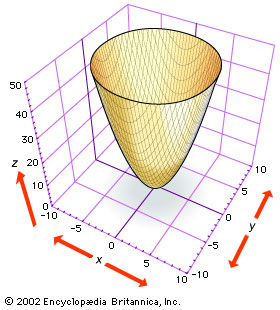
\includegraphics[width=0.3\textwidth]{paraboloid.jpg}
  \end{center}
  \caption{A Paraboloid}
\end{wrapfigure}


By way of some clever linear algebra tricks, one finds that the solution $x$ to the system $Tx=b$, which often arises in PDEs is the coordinate which corresponds to the minimum of the paraboloid. Then one rephrases the problem in terms of gradients (conjugate gradients, actually) and takes a series of steps with ever increasing accuracy to the acutal solution $x$. Note that this is a bit different from the Euler Method in that the Euler Method is a repeated iteration of $T$ upon $x$, which yields $b$. The conjugate gradient method presupposes that you are after an $x$ which will give you a $b$ which you are already interested in. For example, CG is often introduced with the Laplace Equation in which one tries to find the vector $\phi$ which satisfies :
\begin{equation}
0 = \frac{\partial^2}{\partial x^2}\phi + \frac{\partial^2}{\partial y^2}\phi + \frac{\partial^2}{\partial z^2}\phi
\end{equation}

at all of the points in a mesh. The Laplace equation most frequently arises in fluid dynamics, electromagnetics, and thermodynamics when one wants to find the steady state distribution of [charges/temperature/energy] given certain imposed conditions (in this case zero on the boundary). If the boundary condition is non-zero, then the equation is referred to as Poisson's Equation. A very interesting facet of CG is that you are guaranteed to reach the solution vector $x$ in a maximum of $n$ steps, where $n$ is the width of the square matrix $T$.

The details of the algorithm are somewhat involved, but here it is, in figure 5, in all of its beautiful simplicity\footnote{Thanks to \url{http://komarix.org/ac/papers/thesis/thesis_html/img85.png}}. UYOU MAY NOTICE THAT THE ITERATIVE MULTIPLICATIONS ARE NOT THE SAME AS IN THE FORWEARD EULER METHOD. THESE are nested inside other operations.

PRECONDITIONING, AND HOW IT INTRODUCES MORE STEPS, MORE ERROR PRONE STEPS INTO THE CALCULATION

\begin{figure}
\centering
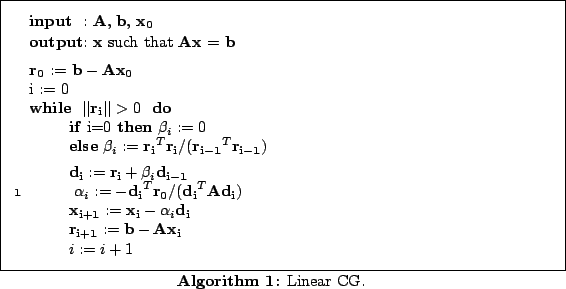
\includegraphics[scale=0.5]{cg.png}
\caption{The CG Algorithm}
\end{figure}

\section{Error Analysis}
The aforementioned algorithms have certain parameters associated with their stability. For example, it is intuitively clear that a finer mesh and a smaller time step will give you a better approximation of heat flow when one uses the Euler Method. What is not intuitively clear is that floating point errors will ruin the solution is one  does not choose the time step and mesh-fine-ness in a specific way. One can also show that, in general, all of the iterated solvers we have seen in this paper can, under certain circumstances, magnify single soft errors and spread the error throughout a solution. In this section we will look first at a traditional method of error analysis for iterative solvers, then look at some of the new work in the field, and then investigate their overlap.

\subsection{Von Neumann Stability Analysis}
John Von Neumann is a very important figure in computer science and mathematics. He invented a method of error analysis for a subset of finite difference schemes for the solution, including the Forward Euler Method which was presented at the beginning of this paper. We made mention of the fact that the Forward Euler Method provides the correct solution of the heat equation only if the time step and the division of the domain satisfies a condition. We will now provide that condition.

EXPLAIN MORE ABOUT WHY WE ASSUME THIS FORM FOR THE SOLUTION.

We expect the numerical solution to converge to the real solution. Therefore, we expect the space between $u^{n+1}$ and $u^n$, the $n^{th}$ and $(n+1)^{th}$ solutions to go to zero as $n$ goes to $\infty$. the method consists of approximating the solution to the equation as $T^n_j = \xi^ne^{ikj\Delta x}$. $j\Delta x$ describes the position in the grid, and $n$ is the current time. For this analysis we are ignoring the $k$, which deals with a Fourier Series expansion of the solution and is beyond the scope of this paper. Then we plug all of these terms into the heat equation.

We want the solution to converge. Therefore, we need $|\xi|\le 1$ Since the exponential term has magnitude 1, if $|\xi|>1$, $T\to\infty$ as the number of iterations grows.
\begin{gather}
\frac{u(x, t + \Delta t) - u(x, t)}{\Delta t} = \frac{u(x + \Delta x, t) - 2u(x, t) + u(x - \Delta x, t)}{\Delta x^2}\\
\frac{T^{n+1}_j - T^n_j}{\Delta t} = \frac{T^n_{j+1} - 2T_j^n + T_{j-1}^n}{\Delta x^2}\\
\frac{\xi^{n+1}e^{ikj\Delta x} - \xi^ne^{ikj\Delta x}}{\Delta t} = \frac{\xi^n(e^{ik(j+1)\Delta x} - 2e^{ikj\Delta x} + e^{ik(j-1)\Delta x})}{\Delta x^2}\\
\xi - 1 = \frac{\Delta t}{\Delta x^2}(e^{ik\Delta x} - 2 + e^{-ik\Delta x})\\
\xi = 1 + 2\frac{\Delta t}{\Delta x^2}(cos(k\Delta x) - 1)\\
\textrm{and since}\\
-1\le cos(k\Delta x) - 1 \le 0\\
\textrm{we need}\\
2\frac{\Delta t}{\Delta x^2} \le 1 \implies \frac{\Delta t}{\Delta x ^ 2} \le \frac12
\end{gather} 
The Von Neumann Stability analysis accoutns for numerical instability of an algorithm due to any sort of error, including rounding errors coming from floating point arithmetic.
\subsection{Error Propogation}
In their paper they discuss how soft errors can ruin a solution
\subsection{Characterizing $\beta$}
These conflicting error analyses lead us to my \textbf{FIRST THESIS RESEARCH PROPOSAL}, which is to investigate the relationship between the Von Neumann and Shantharam error analyses. The latter does not prove divergence of the iterative solution for matrices with large two norms, as the beta term in the error magnitude statement is not accounted for. Indeed, this beta term is significant in cases such as the Forward Euler Method, which diverges long before the maximum row 2 norm exceeds 1. 

Interest in finding a matrix whose maximum row 2 norm exceeds 1 and yet due to the unaccounted for beta term does not diverge. There is a buffering from the 

These two error analyses may not be comparable one hundred percent 

\section{Error Detection}
\subsection{Matrix Check Summing}
Thusfar we have only dealt with the how errors propogate. The real issue is, ``How do we detect the errors when they are introduced, and before they infect our entire computation?" One of the leading techniques to this end 
\subsection{Sparse Matrix Check Summing}
how to do it, how it differs from dense checksumming, and how to improve it.
Adding intermediate check sums. When is this favorable?

\section{Inherently Fault Tolerant Algorithms for Iterative Matrix Multiplication.}

\begin{thebibliography}{1}
\bibitem{FaultTolIt} Bridges, P. et. al. \emph{Fault-tolerant linear solvers via selective reliablity}\url{http://arxiv.org/pdf/1206.1390.pdf} June 8 2012.

\bibitem{ConvCondition} Broyden \emph{On Convergence Criteria for the Method of Successive Over Relaxation} \url{http://www.ams.org/journals/mcom/1964-18-085/S0025-5718-1964-0158527-2/S0025-5718-1964-0158527-2.pdf}

\bibitem{DenseSolver} Du., P. \emph{High Performance Dense Linear System Solver
with Soft Error Resilience}\url{http://www.sciencedirect.com/science/article/pii/S1877050912001445}

\bibitem{EulerGPU} He, X. et. al., \emph{Solving Two Dimensional Euler Equations on the GPU}, Parallel Computational Fluid Dynamics Conference (ParCFD2013)

\bibitem{} Malkowski, K. \emph{Analyzing the soft error resilience of linear solvers on multicore multiprocessors} \url{http://ieeexplore.ieee.org/xpl/login.jsp?tp=&arnumber=5470411&url=http%3A%2F%2Fieeexplore.ieee.org%2Fxpls%2Fabs_all.jsp%3Farnumber%3D5470411}

\bibitem{Self Stab} Sao, P. \emph{Self-stabilizing iterative solvers} \url{http://dl.acm.org/citation.cfm?id=2530272} 2013

\bibitem{OrigPaper} Shantharam M. et. al., \emph{Characterizing the impact of soft errors on iterative methods in scientific computing
}, \url{http://dl.acm.org/citation.cfm?id=1995922}

\bibitem{FaultTolCG} Shantharam M. et. al. \emph{Fault tolerant preconditioned conjugate gradient for sparse linear system solution
}, \url{http://dl.acm.org/citation.cfm?id=2304576.2304588&coll=DL&dl=GUIDE&CFID=581632805&CFTOKEN=50431262}, 2012.

\bibitem{ConjGrad} Shewchuck, J.S., \emph{An Introduction to the Conjugate Gradient Method Without the Agonizing Pain}, \url{http://www.cs.cmu.edu/~quake-papers/painless-conjugate-gradient.pdf} August 4th, 1994.

\bibitem{} Young, David. \emph{Iterative Methods for Solving Partial Difference Equations of Elliptic Type} \url{https://web.stanford.edu/class/cme324/young.pdf} 1950
\bibitem{InnerOuter}  Zheng, Z. et. al., \emph{Fault Tolerance in an Inner Outer Solver}, \url{http://www.vecpar.org/papers/vecpar2014_submission_4.pdf}

\end{thebibliography}
\end{document}